
%%%%%%%%%%%%%%%%%%%%%%% file typeinst.tex %%%%%%%%%%%%%%%%%%%%%%%%%
%
% This is the LaTeX source for the instructions to authors using
% the LaTeX document class 'llncs.cls' for contributions to
% the Lecture Notes in Computer Sciences series.
% http://www.springer.com/lncs       Springer Heidelberg 2006/05/04
%
% It may be used as a template for your own input - copy it
% to a new file with a new name and use it as the basis
% for your article.
%
% NB: the document class 'llncs' has its own and detailed documentation, see
% ftp://ftp.springer.de/data/pubftp/pub/tex/latex/llncs/latex2e/llncsdoc.pdf
%
%%%%%%%%%%%%%%%%%%%%%%%%%%%%%%%%%%%%%%%%%%%%%%%%%%%%%%%%%%%%%%%%%%%


\documentclass[runningheads,a4paper]{llncs}

\usepackage{amssymb}
\setcounter{tocdepth}{3}
\usepackage{graphicx}
\usepackage{times,amsmath,epsfig}
\usepackage[linesnumbered,ruled,vlined]{algorithm2e}
\usepackage{subfigure}

\usepackage{url}
%\urldef{\mailsa}\path|{alfred.hofmann, ursula.barth, ingrid.haas, frank.holzwarth,|
%\urldef{\mailsb}\path|anna.kramer, leonie.kunz, christine.reiss, nicole.sator,|
%\urldef{\mailsc}\path|erika.siebert-cole, peter.strasser, lncs}@springer.com|
%\newcommand{\keywords}[1]{\par\addvspace\baselineskip
%\noindent\keywordname\enspace\ignorespaces#1}


\begin{document}

\mainmatter  % start of an individual contribution

\pagestyle{empty}

% first the title is needed
\title{Mining Probabilistic High Utility Itemsets in Uncertain Databases}

% a short form should be given in case it is too long for the running head
%\titlerunning{Lecture Notes in Computer Science: Authors' Instructions}

% the name(s) of the author(s) follow(s) next
%
% NB: Chinese authors should write their first names(s) in front of
% their surnames. This ensures that the names appear correctly in
% the running heads and the author index.
%
\author{Yuqing Lan
%\thanks{Please note that the LNCS Editorial assumes that all authors have used
%the western naming convention, with given names preceding surnames. This determines
%the structure of the names in the running heads and the author index.}%
\and Yang Wang \and Shengwei Yi \and Dan Yu \and Simin Yu
}

%
%\authorrunning{Lecture Notes in Computer Science: Authors' Instructions}
% (feature abused for this document to repeat the title also on left hand pages)

% the affiliations are given next; don't give your e-mail address
% unless you accept that it will be published

\institute{School of Computer Science and Engineering, Beihang University, China\\
\email{\{lanyuqing, yangwang, yishengwei, yudan, siminyu\}@buaa.edu.cn}
}


%
% NB: a more complex sample for affiliations and the mapping to the
% corresponding authors can be found in the file "llncs.dem"
% (search for the string "\mainmatter" where a contribution starts).
% "llncs.dem" accompanies the document class "llncs.cls".
%

%\toctitle{Lecture Notes in Computer Science}
%\tocauthor{Authors' Instructions}
\maketitle


\begin{abstract}

Recently, with the growing popularity of Internet of Things (IoT) and pervasive computing, a large amount of uncertain data, i.e. RFID data, sensor data, real-time monitoring data, etc., has been collected. As one of the most fundamental issues of uncertain data mining, the problem of mining uncertain frequent itemsets has attracted much attention in the database and data mining communities. Although some efficient approaches of mining uncertain frequent itemsets have been proposed, most of them only consider each item in one transaction as a random variable following the binary distribution and ignore the unit values of items in the real scenarios. In this paper, we focus on the problem of \textit{\underline{m}ining \underline{p}robabilistic \underline{h}igh \underline{u}tility itemsets in uncertain databases} (MPHU), in which each item has a unit value. In order to solve the MPHU problem, we propose a novel mining framework, called UUIM, which not only includes an efficient mining algorithm but also contains an effective pruning technique. Extensive experiments on both real and synthetic datasets verify the effectiveness and efficiency of proposed solutions.

%\keywords{Correlated Uncertain Graphs, Shortest Path, Sampling}
\end{abstract}


\section{Introduction}
\label{sec:intro}

\vspace{-0.3cm}

Recently, with the growing popularity of Internet of Things (IoT) and pervasive computing, a large amount of uncertain data, i.e. RFID data, sensor data, real-time monitoring data, etc., has been collected. As one of the most fundamental issues of uncertain data mining, the problem of mining uncertain frequent itemsets has attracted much attention in the database and data mining communities. Although some efficient approaches of mining uncertain frequent itemsets have been proposed, most of them only consider each item in one transaction as a random variable following the binary distribution and ignore the unit values of items in the real scenarios.  In recommender system (e.g. music, video) analysis, mining frequent itemsets from an uncertain database refers to the discovery of itemsets which may frequently appear together in the records (transactions). However, in these works, the unit values (profits) of items are not considered in their frameworks of uncertain frequent itemsets mining. Hence, it cannot satisfy the requirement of a user who is interested in discovering itemsets with high enjoyment values. For example, Table~\ref{tab:song} shows some songs and their utility values. The utility value of each song is scored by all the persons listened to it according to their preference degree to the song. Table ~\ref{tab:record} are the listening records of some users showing which songs they listened to and the probability they like them. Namely, the first line in Table ~\ref{tab:record} means Jack listened 4 songs in Table ~\ref{tab:song}, and the probability he likes these songs are 0.8, 0.8, 0.7, and 0.7. When songs are recommended, not only the frequency of songs in records of different user should be considered, but the popularity of songs should also be taken into account. In view of this, utility mining is a necessary topic in data mining for discovering itemsets with high utility, such as values (profits), in uncertain databases.

\begin{table}[htbp]
\vspace{-0.2cm}
  \centering
  \caption{\small{A Table of Songs}}
\vspace{-0.1cm}
  \label{tab:song}
  \begin{tabular}{|c|c|c|}
    \hline
    \bfseries {ID} & \bfseries {Song Name} & \bfseries {Score} \\
    \hline
    A & Big Big World & 3 \\
    \hline
    B & Someone Like You & 4 \\
    \hline
    C & Don��t You Remember & 1 \\
    \hline
    D & My Love & 1 \\
    \hline
    E & Time to say goodbye & 8 \\
    \hline
    F & Right Here Waiting & 2 \\
    \hline
    G & Can You & 1 \\
    \hline
    %soc-Epinions1 & 75,879 & 508,837 \\
%    \hline
    \end{tabular}
\vspace{-0.4cm}
\end{table}

\begin{table}[htbp]
\vspace{-0.2cm}
  \centering
  \caption{\small{A Table of Records}}
\vspace{-0.1cm}
  \label{tab:record}
  \begin{tabular}{|c|c|}
    \hline
    \bfseries {User} & \bfseries {Record and matching analysis} \\
    \hline
    Jack & (A, 0.8) (B, 0.8) (C, 0.7) (D, 0.7) \\
    \hline
    Rose & (A, 0.9) (C, 0.8) (G, 0.8) \\
    \hline
    Tom & (A, 0.6) (B, 0.7) (C, 0.6) (D, 0.5) (E, 0.8) (F, 0.5) \\
    \hline
    Peter & (B, 0.7) (C, 0.8) (D, 0.5) \\
    \hline
    Linda & (B, 0.8) (C, 0.7) (F, 0.4) \\
    \hline
    %soc-Epinions1 & 75,879 & 508,837 \\
%    \hline
    \end{tabular}
\vspace{-0.4cm}
\end{table}

Mining high utility itemsets from the databases refers to finding the itemsets with high utilities. The basic meaning of utility is the interestingness / importance / profitability of an item to the users. Before finding high utility itemsets over uncertain databases, the definition of the high utility itemset is the most essential issue. In deterministic data, the utility of items in a transaction database consists of two aspects: (1) the importance of distinct items, which is called external utility, and (2) the importance of the items in the transaction, which is called internal utility. The utility of an itemset is defined as the external utility multiplied by the internal utility. An itemset is called a high utility itemset if its utility is not less than a user-specified threshold. The definition of a high utility itemset over uncertain data has two different semantic explanations: expected support-based high utility itemset and probabilistic high utility itemset. However, the two definitions are different on using the random variable to define high utility itemsets. In the definition of the expected support-based high utility itemset, the expectation of the utility of an itemset is defined as the expected utility of this itemset, in which an itemset is of high utility if and only if the expected utility of such itemset is not less than a specified minimum expected utility threshold, $min\_util$. In the definition of probabilistic utility itemset, the probability that the utility of an itemset is not less than the threshold is defined the high utility probability of an itemset, in which an itemset is of high utility if and only if the high utility probability of such itemset is larger than a given probabilistic threshold.

Mining high utility itemsets from uncertain databases is an important task which is essential to a wide range of applications such as recommender system analysis, Internet of Things (IoT) and biomedical applications. The definition of probabilistic high utility itemset includes the complete probability distribution of the utility of an itemset. Although the expectation is known as an important statistic, it cannot show the complete probability distribution. Hence, we mainly discuss mining probabilistic high utility itemsets in this paper.


\vspace{-0.5cm}
\subsubsection*{To sum up, we make the following contributions:}

\begin{itemize}
\vspace{-0.2cm}
\item	To the best of our knowledge, this is the first work to formulate the problem of mining probabilistic high utility itemsets in uncertain databases (MPHU).
\item   Due to the challenges from utility constraints, we propose a novel mining framework, called UUH-mine, which not only includes an efficient mining algorithm but also contains an effective pruning technique.
\item   We verify the effectiveness and efficiency of the proposed methods through extensive experiments on real and synthetic datasets.
\vspace{-0.2cm}
\end{itemize}

The rest of the paper is organized as follows. Preliminaries and our problem formulation are introduced in Section 2. In Section 3, we present a novel mining framework, called UUH-mine. Based on this framework, an efficient mining algorithm and an effective pruning technique is devised in Section 4. In Section 5, experimental studies on both real and synthetic datasets are reported. In Section 6, we review the existing works. Finally, we conclude this paper in Section 7.

\section{Preliminaries and Problem Definitions}
\label{sec:model-ProState}

\vspace{-0.3cm}
In this section, we first introduce some basic concepts and then define the problem of mining probabilistic high utility itemsets in uncertain databases.

\vspace{-0.3cm}
\subsection{Preliminaries}
\label{sec:sec:model}

We first review the classical problem of frequent pattern mining in deterministic databases.

Given a finite set of items $I = \{i_1,i_2,...,i_n\}$. An itemset X is a subset of items, i.e., $X \subseteq I$. For the sake of brevity, an itemset $X = \{i_1,i_2,...,i_m\}$ is also denoted as $X = i_1i_2...i_m$. A transaction $T = (tid, Y)$, where $tid$ is a transaction-id and $Y$ is an itemset. A transaction $T = (tid, Y)$ is said to contain itemset $X$ if and only if $X \subseteq Y$. A transaction database $D$ is a set of transactions. The number of transactions in $D$ containing itemset $X$ is called the support of $X$, denoted as $sup(X)$. Given a transaction database $D$ and a support threshold $min\_sup$, an itemset $X$ is a frequent pattern, or a pattern in short, if and only if $sup(X) \geq min\_sup$.

The problem of frequent pattern mining is to find the complete set of frequent patterns in a given transaction database with respect to a given support threshold.

In the problem of high utility pattern mining, each item $i_p$($1\leq p\leq n$) has a unit profit $p(i_p)$, and each item $i_p$ in the transaction $T_d$ is associated with a quantity $q(i_p,T_d)$, that is, the purchased number of $i_p$ in $T_d$. The utility of an item $i_p$ in the transaction $T_d$ is denoted as $u(i_p,T_d) = p(i_p)\times q(i_p, T_d)$. The utility of an itemset $X$ in $T_d$ is denoted as $u(X,T_d) = \sum_{i_p\in X\wedge X\subseteq T_d}u(i_p,T_d)$. The utility of an itemset $X$ in $D$ is denoted as $u(X)$ and defined as $\sum_{X\subseteq T_d\wedge T_d\in D}u(X,T_d)$. An itemset is called a high utility itemset if its utility is not less than a user-specified minimum utility threshold, which is denoted as $min\_util$. Otherwise, it is called a low utility itemset.

Given a transaction database $D$ and a user-specified minimum utility threshold $min\_util$, mining high utility itemsets from the transaction database is equivalent to discovering from $D$ all itemsets whose utilities are no less than $min\_util$.

All the above mentioned problems are based on the deterministic databases. When mining high utility itemsets in uncertain databases, there will be lots of differences.

\vspace{-0.2cm}
\subsection{Problem Definitions}
\label{sec:sec:pro-state}
\vspace{-0.2cm}

In this subsection, we give several basic definitions about mining high utility itemsets over uncertain databases.

Let $I =\{i_1,i_2,...,i_n\}$ be a set of distinct items. Each item $i_p$ has a unit value $v(i_p)$. We name a non-empty subset, $X$, of $I$ as an itemset. For brevity, we use $X = x_1x_2...x_n$ to denote itemset $X = \{x_1,x_2,...x_n\}$. $X$ is a $l$ - item set if it has $l$ items. Given an uncertain transaction database $UD$, each transaction is denoted as $< tid, Y >$, where $tid$ is the transaction identifier, and $Y = \{y_1(p_1),y_2(p_2),...,y_n(p_n)\}$. $Y$ contains $n$ units. Each unit has an item $y_i$ and probability $p_i$, denoting the possibility of item $y_i$ appearing in the $tid$ tuple. The number of transactions containing $X$ in $UD$ is a random variable, denoted as $sup(X)$. Given $UD$, the expected support-based high utility itemsets and probabilistic high utility itemsets are defined as follows.

\vspace{-0.3cm}
\begin{definition}[Expected Support]
\label{def:ES}
Given an uncertain transaction database $UD$ which includes $N$ transactions, and an itemset $X$, the expected support of $X$ is:
\end{definition}
\vspace{-0.3cm}

\vspace{-0.2cm}
\begin{equation}
\label{eq:esup}
esup(X)=
\sum_{i = 1}^{N}
p_i(X)
\end{equation}

\begin{table}[htbp]
\vspace{-0.2cm}
  \centering
  \caption{\small{An Uncertain Database}}
\vspace{-0.1cm}
  \label{tab:ud}
  \begin{tabular}{|c|c|}
    \hline
    \bfseries {TID} & \bfseries {Transaction} \\
    \hline
    $T_1$ & (A, 0.8) (B, 0.8) (C, 0.7) (D, 0.7) \\
    \hline
    $T_2$ & (A, 0.9) (C, 0.8) (G, 0.8) \\
    \hline
    $T_3$ & (A, 0.6) (B, 0.7) (C, 0.6) (D, 0.5) (E, 0.8) (F, 0.5) \\
    \hline
    $T_4$ & (B, 0.7) (C, 0.8) (D, 0.5) \\
    \hline
    $T_5$ & (B, 0.8) (C, 0.7) (F, 0.4) \\
    \hline
    %soc-Epinions1 & 75,879 & 508,837 \\
%    \hline
    \end{tabular}
\vspace{-0.5cm}
\end{table}

\begin{table}[htbp]
\vspace{-0.2cm}
  \centering
  \caption{\small{Value Table}}
\vspace{-0.1cm}
  \label{tab:vt}
  \begin{tabular}{|c|c|c|c|c|c|c|c|}
    \hline
    \bfseries {Item} & \bfseries {A} & \bfseries {B} & \bfseries {C} & \bfseries {D} & \bfseries {E} & \bfseries {F} & \bfseries {G}\\
    \hline
    Value & 3 & 4 & 1 & 1 & 8 & 2 & 1\\
    \hline
    %soc-Epinions1 & 75,879 & 508,837 \\
%    \hline
    \end{tabular}
\vspace{-0.5cm}
\end{table}

Different from deterministic databases, the utility of an itemset $X$ in $T_d$ is denoted as $u(X,T_d)$ and defined as $\sum_{i_p\in X}v(i_p)$ in uncertain databases.

\begin{table}[htbp]
\vspace{-0.2cm}
  \centering
  \caption{\small{The Probability Distribution of sup(A)}}
\vspace{-0.1cm}
  \label{tab:pd}
  \begin{tabular}{|c|c|c|c|c|}
    \hline
    \bfseries {sup(A)} & \bfseries {0} & \bfseries {1} & \bfseries {2} & \bfseries {3}\\
    \hline
    Probability & 0.008 & 0.116 & 0.444 & 0.432\\
    \hline
    %soc-Epinions1 & 75,879 & 508,837 \\
%    \hline
    \end{tabular}
\vspace{-0.4cm}
\end{table}

\vspace{-0.3cm}
\begin{definition}[Expected Utility]
\label{def:EU}
Given an uncertain transaction database $UD$ which includes $N$ transactions, and an itemset $X$, the expected utility of $X$ is:
\end{definition}
\vspace{-0.3cm}

\vspace{-0.2cm}
\begin{equation}
\label{eq:eutil}
EU(X)=
U(X,T_d)\times esup(X)
\end{equation}

\vspace{-0.3cm}
\begin{definition}[Expected Support-based High Utility Itemset]
\label{def:EUI}
Given an uncertain transaction database $UD$ which includes $N$ transactions, and a minimum expected utility ratio, min\_eutil, an itemset X is an expected support-based high utility itemset if and only if $EU(X)\geq N \times min\_eutil$
\end{definition}
\vspace{-0.2cm}

\vspace{-0.2cm}
\begin{definition}[High Utility Probability]
\label{def:HUP}
Given an uncertain transaction database $UD$ which includes $N$ transactions, a minimum utility ratio $min\_util$, and an itemset X, X's high utility probability, denoted as Pr(X), is shown as follows:
\end{definition}
\vspace{-0.3cm}

\vspace{-0.2cm}
\begin{equation}
\label{eq:phu}
Pr(X)=
Pr\{sup(X)\times U(X,T_d)\geq N \times min\_util\}
\end{equation}

\vspace{-0.3cm}
\begin{definition}[Probabilistic High Utility Itemset]
\label{def:PHUI}
Given an uncertain transaction database $UD$ which includes $N$ transactions, a minimum utility ratio $min\_util$, and a probabilistic high utility threshold $put$, an itemset $X$ is a probabilistic high utility itemset if X's high utility probability is larger than the probabilistic high utility threshold, namely,
\end{definition}
\vspace{-0.3cm}

\vspace{-0.2cm}
\begin{equation}
\label{eq:put}
Pr(X)=
Pr\{sup(X)\times U(X,T_d)\geq N \times min\_util\}
\geq put
\end{equation}

\begin{figure}[htbp]
  \centering
  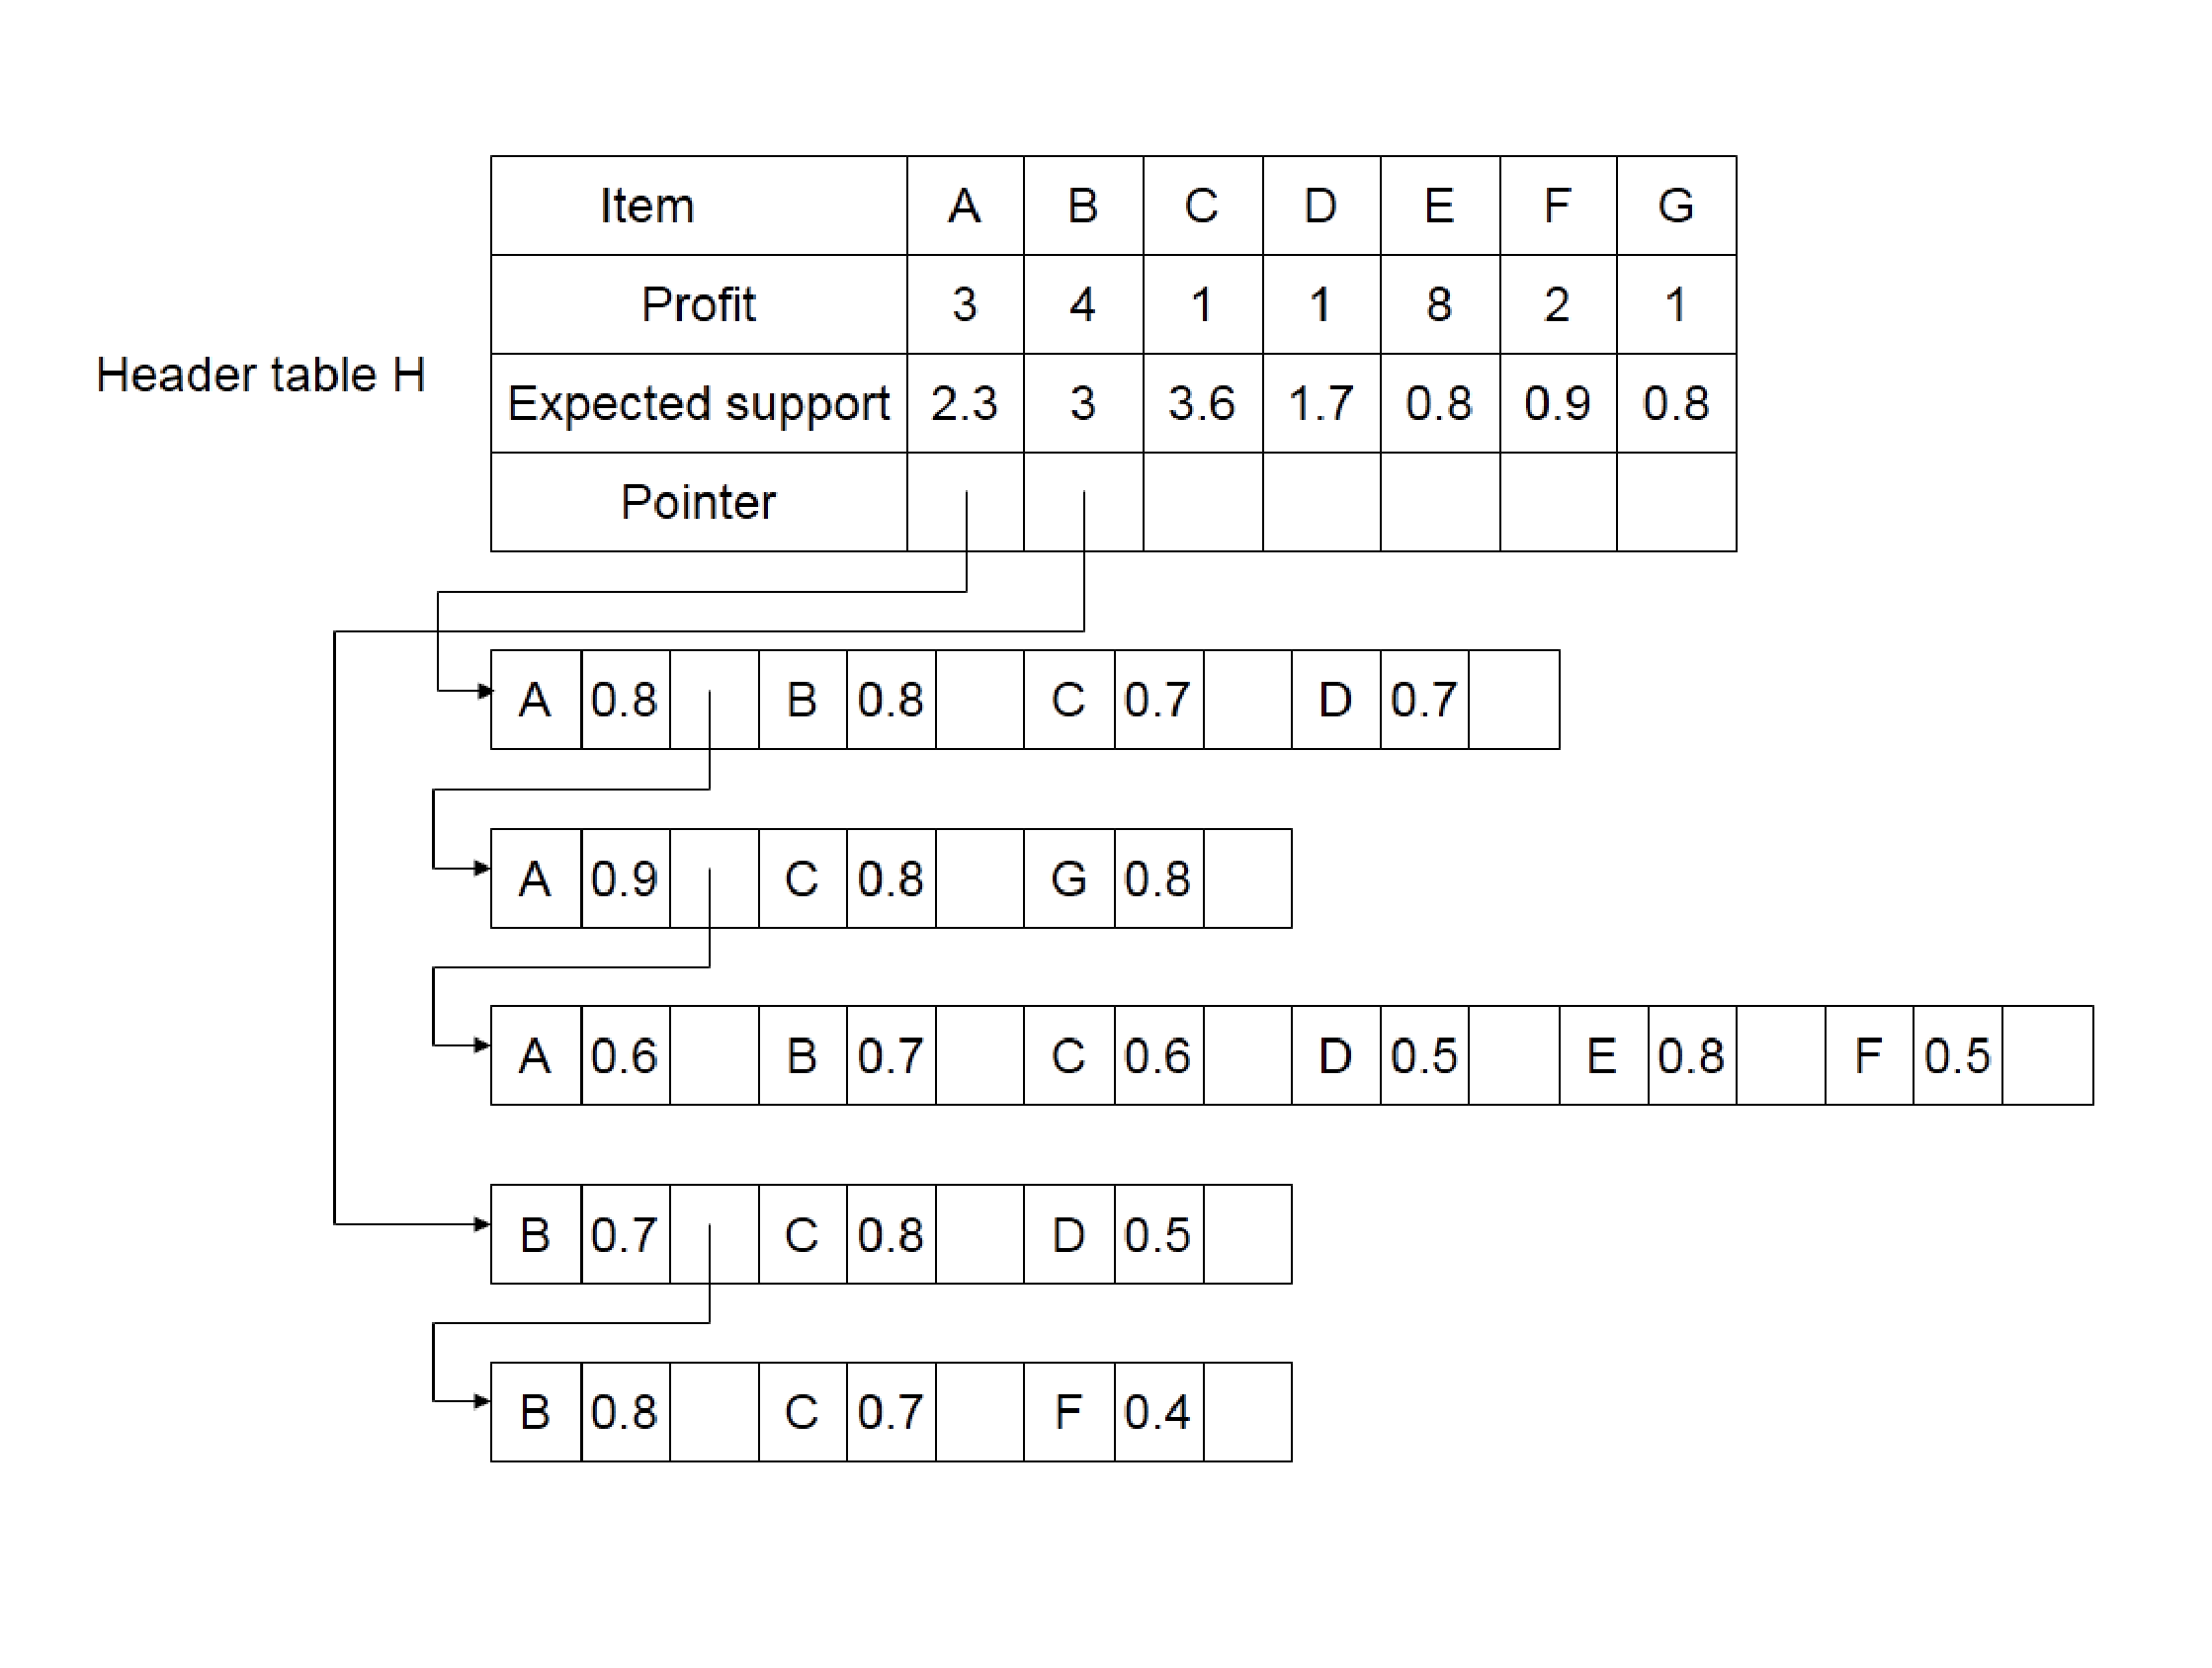
\includegraphics[width=0.99\textwidth]{1.eps}\\
  \caption{UUH-Struct Generated from Table 3}
  \label{fig1}
\end{figure}

Example. Given an uncertain database in Table 5, $min\_util$ = 1 and probabilistic high utility threshold $put$ = 0.9, $sup(A)\geq min\_util \times N \div U(A,T_d)$. So, the high utility probability of A is: $Pr(A) = Pr\{sup(A)\geq 5 \times 1 \div 3\} = Pr\{sup(A)\geq 2\} = Pr\{sup(A) = 2\} + Pr\{sup(A) = 3\} = 0.444 + 0.432 = 0.876 < 0.9 = put$. Thus, \{A\} is not a probabilistic high utility itemset.

We are now able to specify the Mining Probabilistic High Utility Itemsets (MPHU) problem as follows: Given an uncertain transaction database $UD$, a minimum utility threshold $min\_util$ and a probabilistic high utility threshold $put$, the problem of MPHU is to find all probabilistic high utility itemsets in uncertain databases.

\vspace{-0.3cm}
\section{UUH-mine Framework}
\label{sec:base}
\vspace{-0.3cm}

In order to solve the MPHU problem, we propose a novel mining framework, called UUH-Mine, which is based on the divide-and-conquer framework and the depth-first search strategy. The algorithm was extended from the H-Mine algorithm which is classical algorithm in deterministic frequent itemset mining.

UUH-Mine algorithm can be outlined as follows. Firstly, it scans the uncertain database and finds all items. Then, the algorithm builds a head table which contains all items. For each item, the head table stores its four elements: this item, the value, the expected support, and a pointer domain. After building the head table, the algorithm inserts all transactions into the data structure, UUH-Struct.

\begin{figure}[htbp]
  \centering
  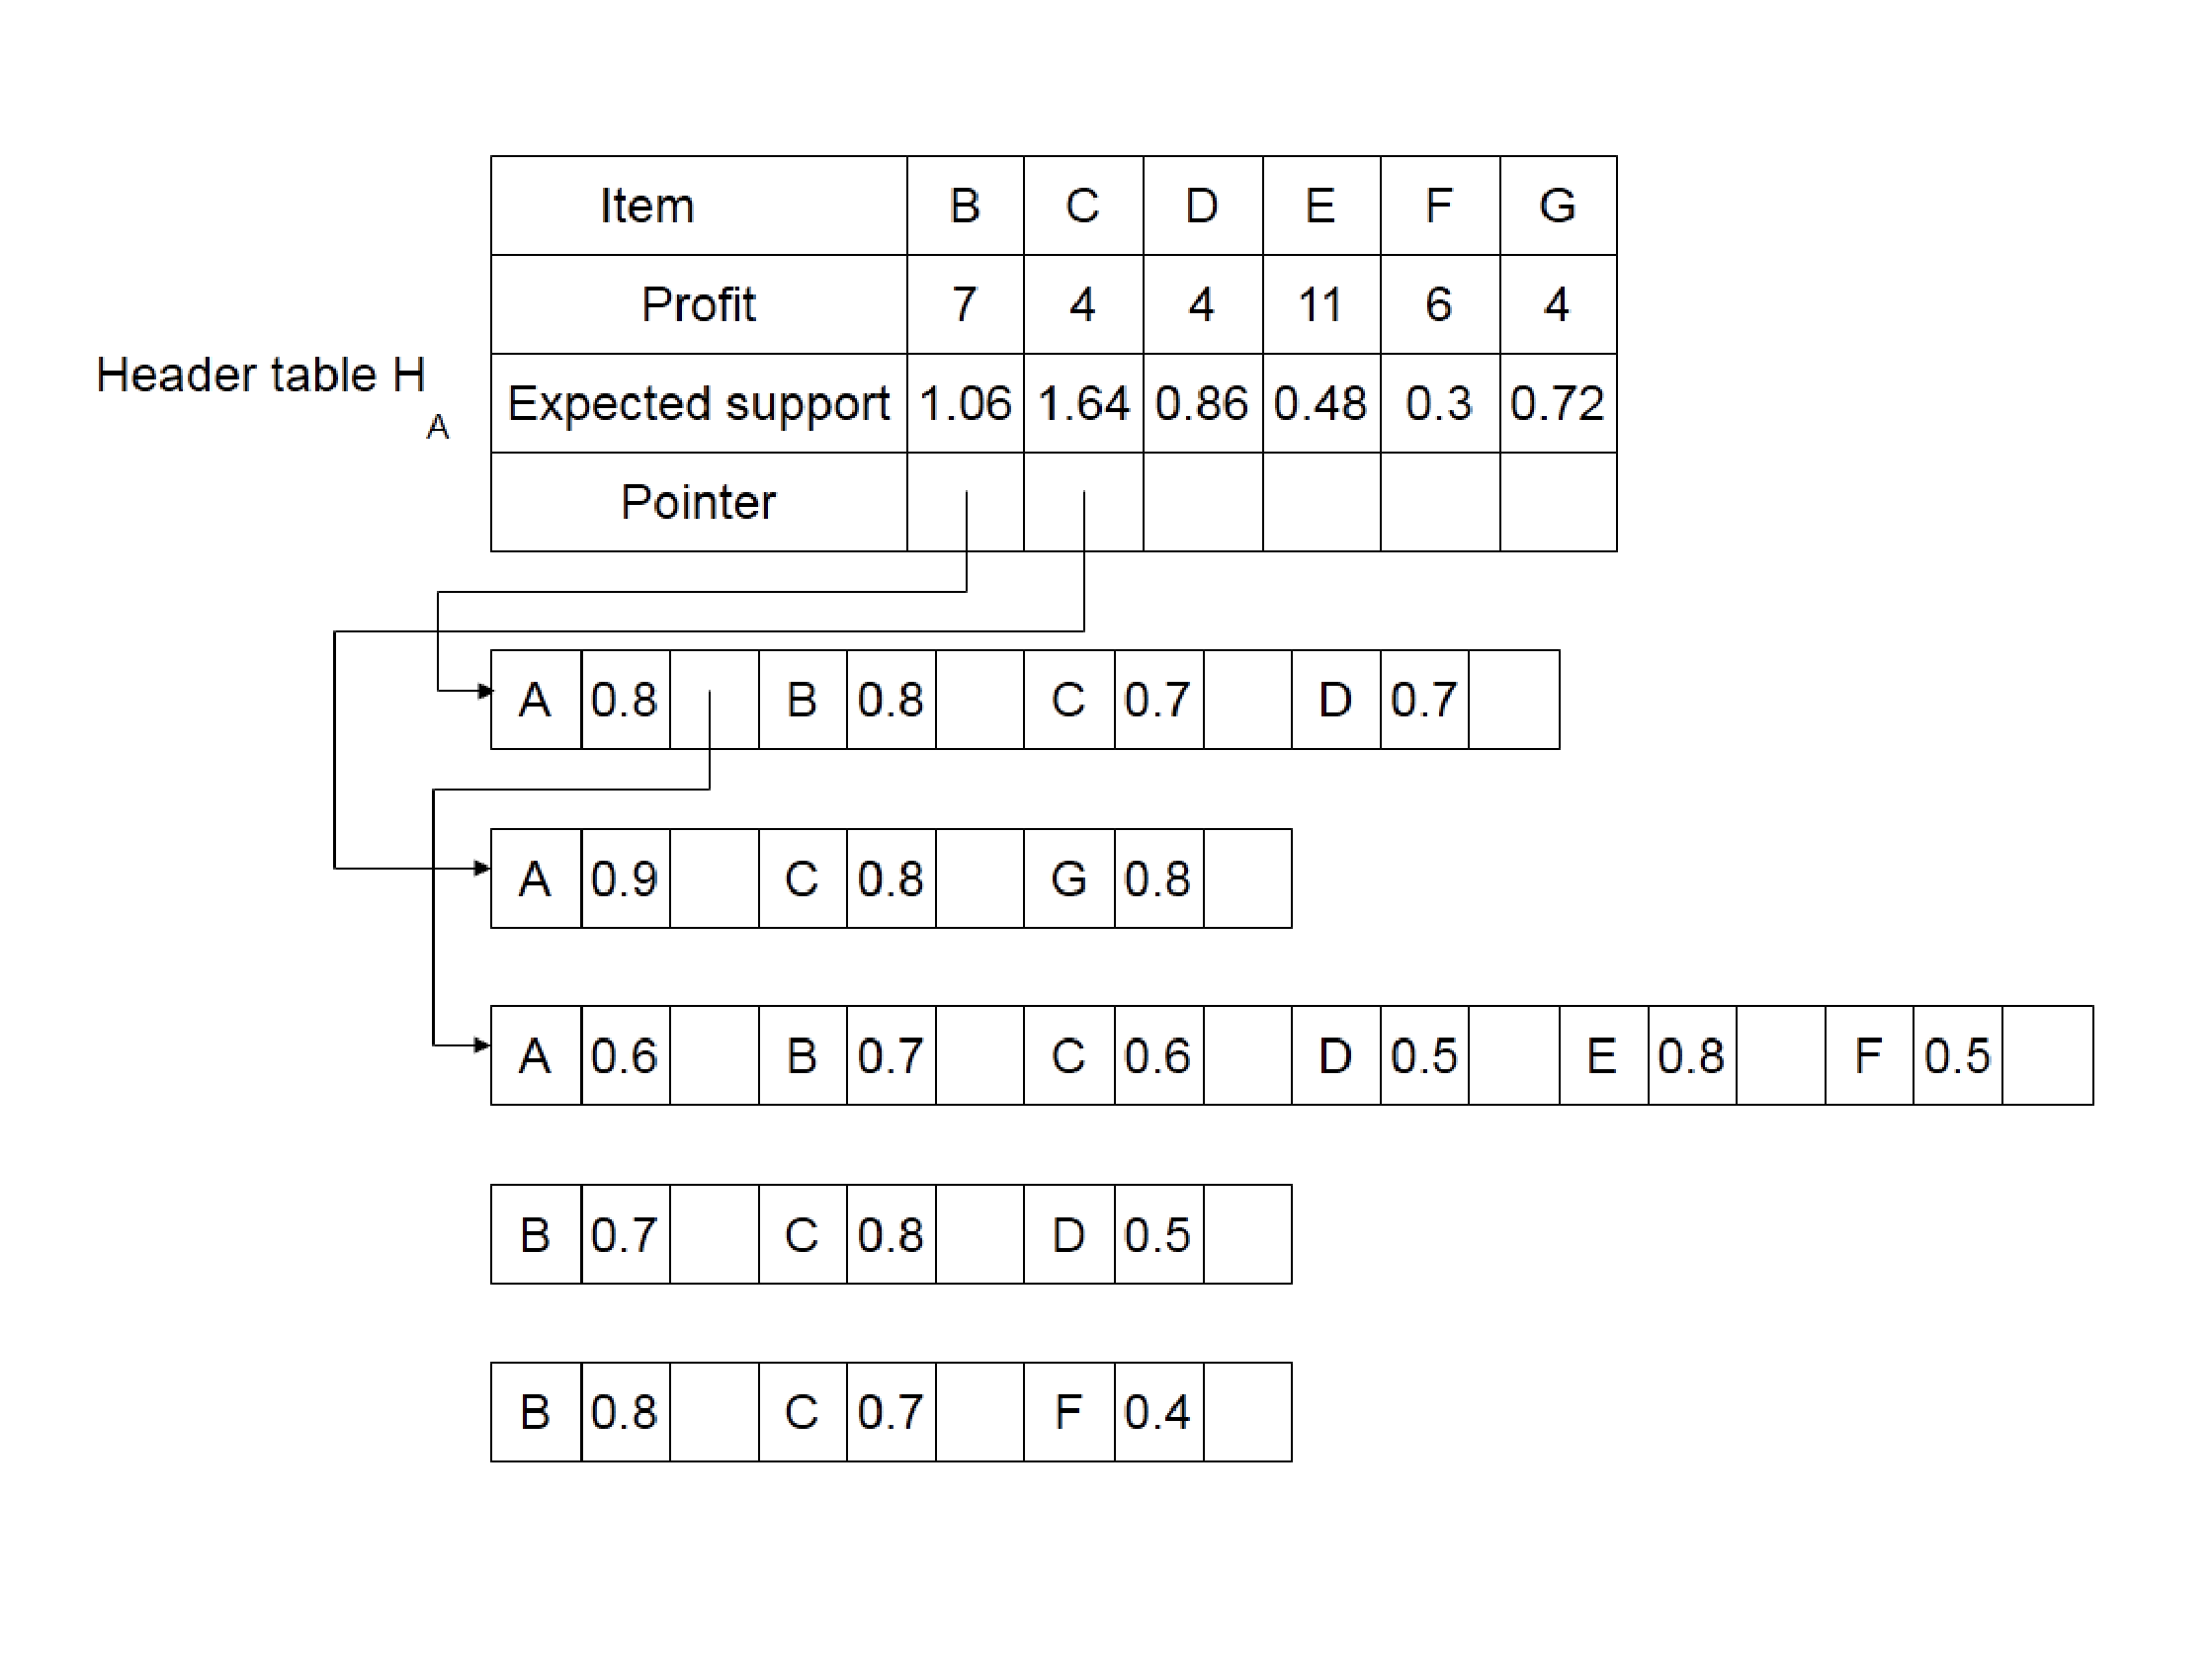
\includegraphics[width=0.99\textwidth]{2.eps}\\
  \caption{UUH-Struct of Head Table of A}
  \label{fig2}
\end{figure}


In this data structure, each item is assigned with its label, its value, its appearing probability and a pointer. The UUH-Struct of Table 3 and Table 4 is shown in Figure 1. After building the global UUH-Struct, the algorithm uses the depth-first strategy to build the head table in Figure 2 where A is the prefix. Then, the algorithm recursively builds the head tables where different itemsets are prefix and generates all the itemsets.

\begin{figure}[htbp]
  \centering
  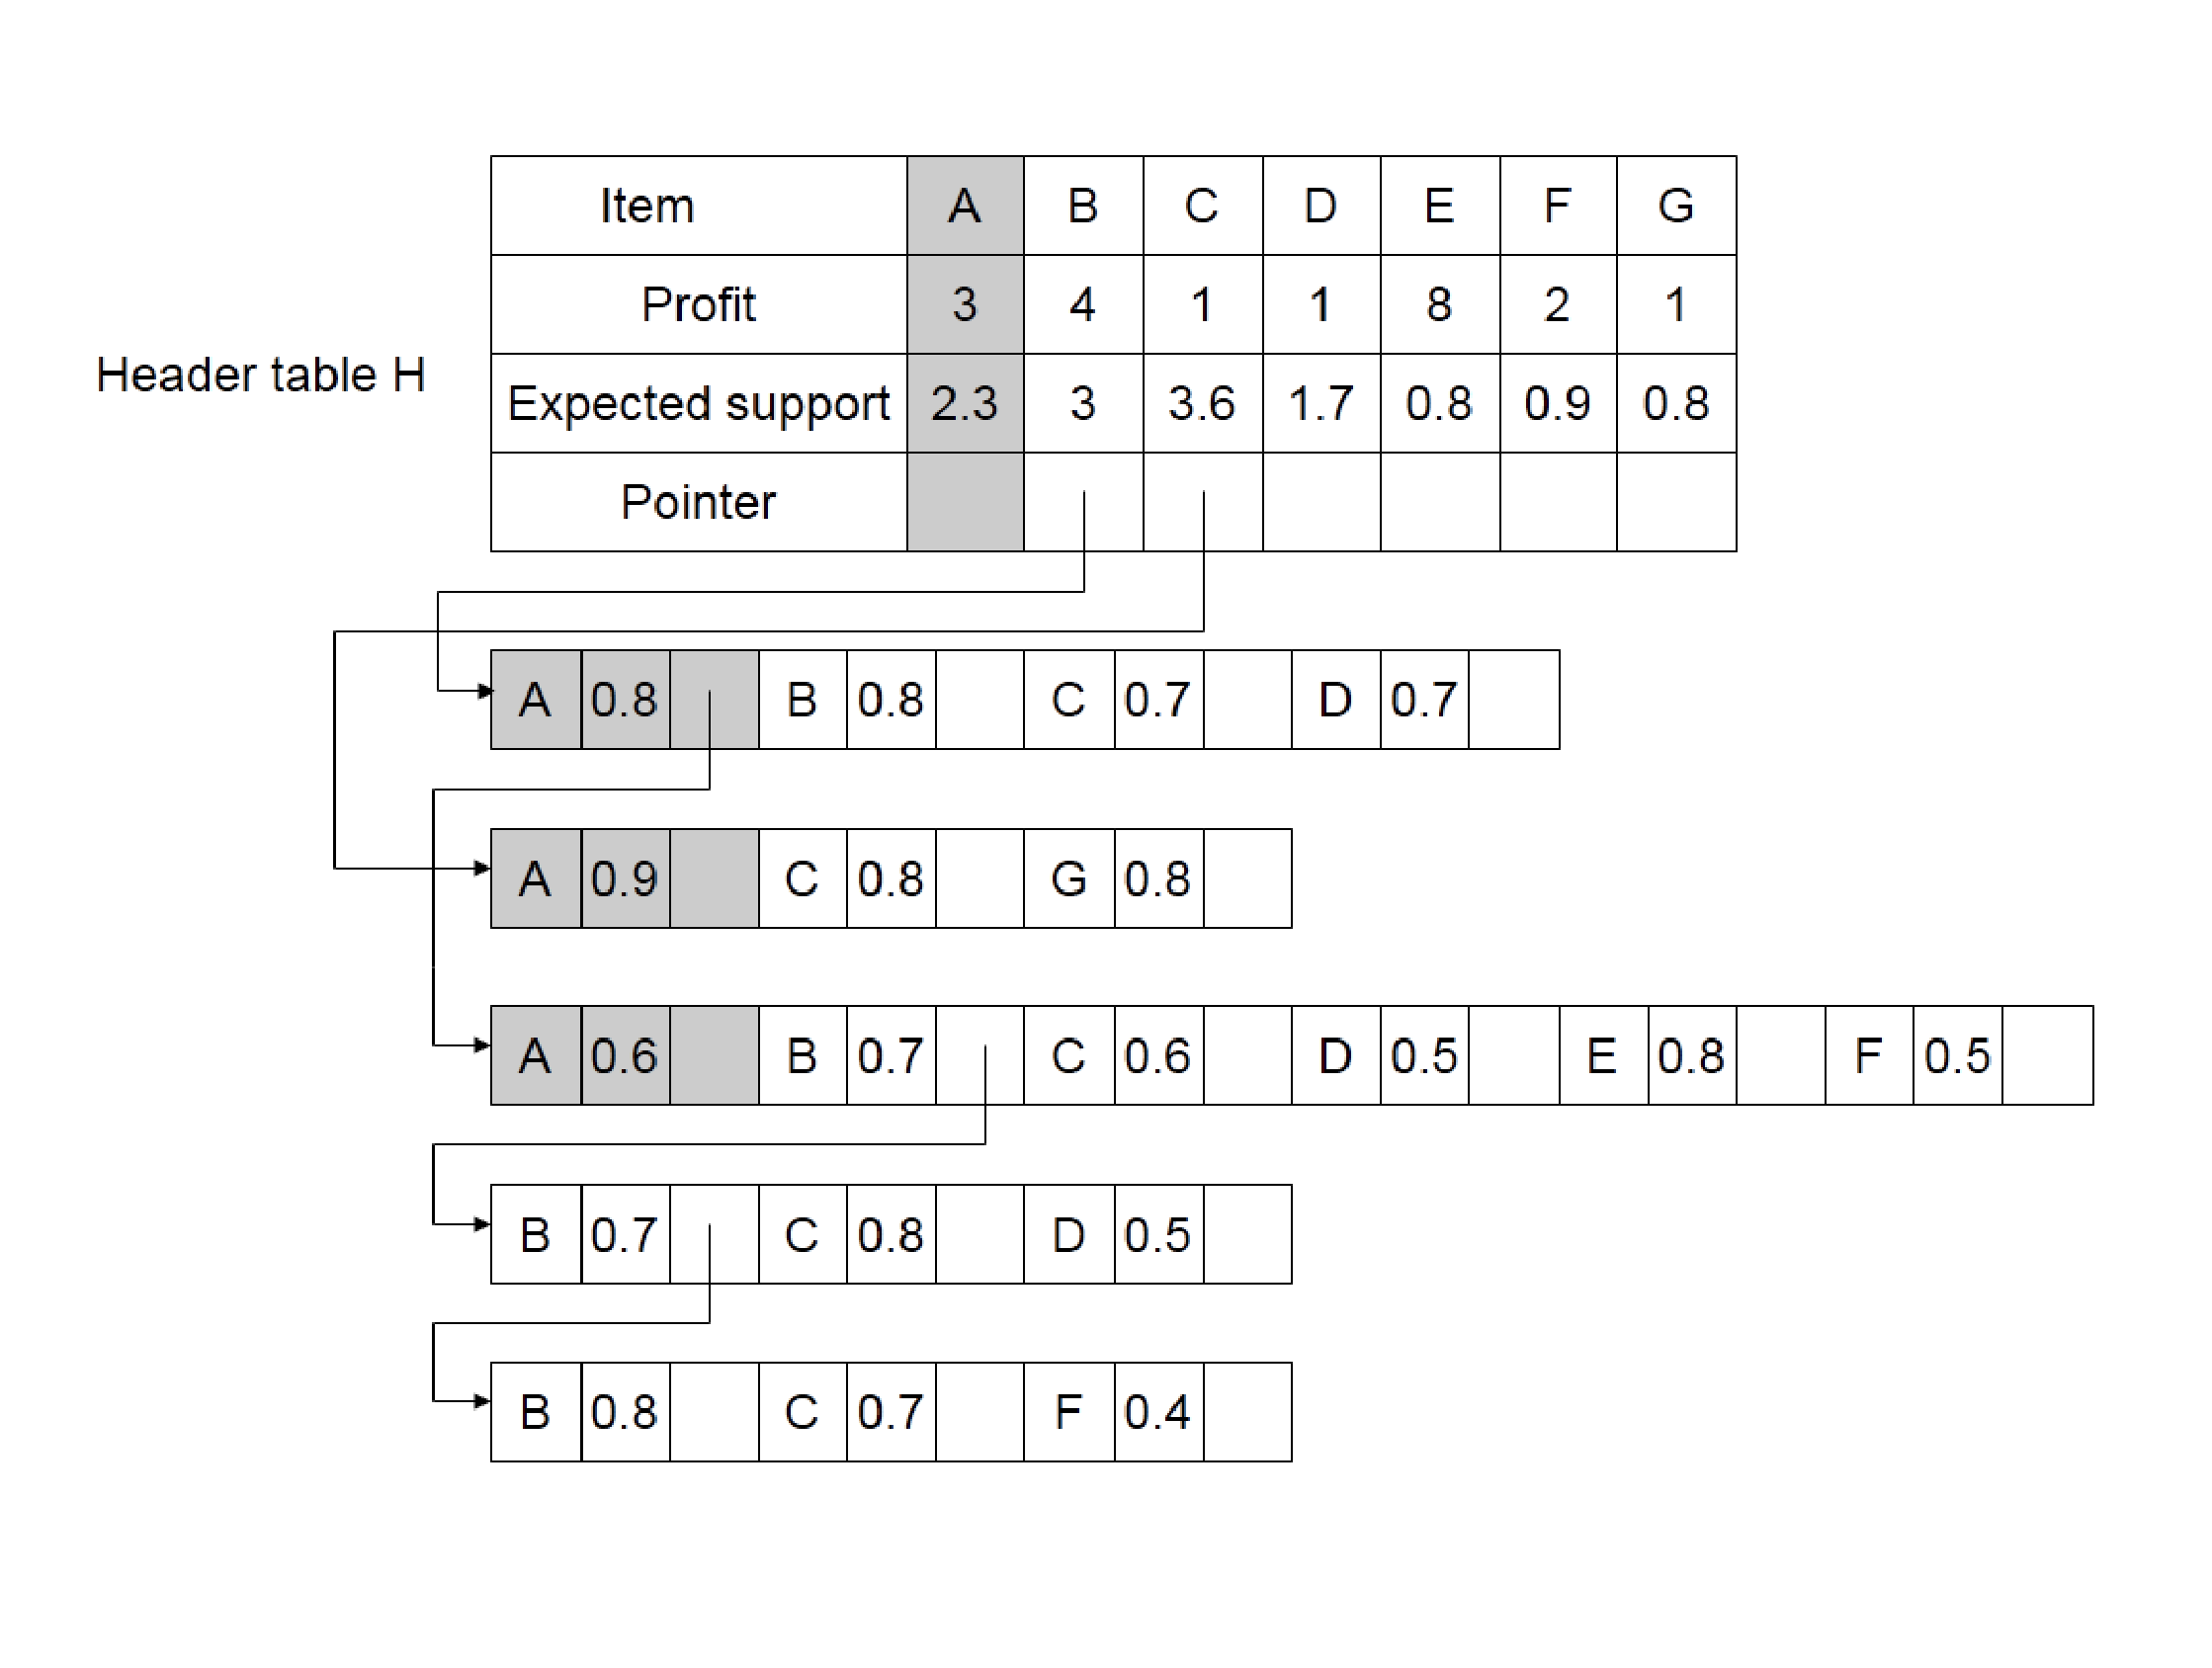
\includegraphics[width=0.99\textwidth]{3.eps}\\
  \caption{UUH-struct after removing item A}
  \label{fig3}
\end{figure}

We use the UUH-Mine framework to find all high utility itemsets from the database through depth first search. However, this UUH-Mine framework needs to traverse all $2^n$ itemsets to find the result, so we must optimize it.

\vspace{-0.4cm}
\section{Optimization Strategies and Algorithms}
\label{sec:impro-samp}
\vspace{-0.2cm}

In this section, we first introduce some optimization Strategies to improve the UUH-Mine framework. Then, we illustrate our UUIM algorithm, which is called Uncertain Utility Itemsets Mining algorithm.

\vspace{-0.2cm}
\subsection{Optimization Strategies}
\label{sec:sec:unequl-pro-samp}


\vspace{-0.2cm}
\begin{definition}[Transaction Maximum Expected Utility]
\label{def:MU}
For the given uncertain transaction T, its transaction maximum expected utility equals to the max expected utility of itemsets it contains, denoted as $MU(T)$:
\end{definition}
\vspace{-0.3cm}

\vspace{-0.2cm}
\begin{equation}
\label{eq:mu}
MU(T)
= max\{EU(X)|X \subset T\}
\end{equation}


For example, the maximum expected utility of transaction 1 is 4.48, and the maximum expected utility of all 16 itemsets contained by transaction 1 is {A, B}, refer to Table 4.

\begin{table}[htbp]
\vspace{-0.2cm}
  \centering
  \caption{\small{Uncertain Database with Maximum Transaction Expected Utility}}
\vspace{-0.1cm}
  \label{tab:mt}
  \begin{tabular}{|c|c|c|}
    \hline
    \bfseries {TID} & \bfseries {Transaction} & \bfseries {MU}\\
    \hline
    $T_1$ & (A, 0.8) (B, 0.8) (C, 0.7) (D, 0.7) & 4.48 \\
    \hline
    $T_2$ & (A, 0.9) (C, 0.8) (G, 0.8) & 2.88 \\
    \hline
    $T_3$ & (A, 0.6) (B, 0.7) (C, 0.6) (D, 0.5) (E, 0.8) (F, 0.5) & 6.72 \\
    \hline
    $T_4$ & (B, 0.7) (C, 0.8) (D, 0.5) & 2.8 \\
    \hline
    $T_5$ & (B, 0.8) (C, 0.7) (F, 0.4) & 3.2 \\
    \hline
    %soc-Epinions1 & 75,879 & 508,837 \\
%    \hline
    \end{tabular}
\vspace{-0.6cm}
\end{table}

In this example, the biggest transaction contains only 6 items, so we can calculate the maximum expected utility of every transaction through exhaustive method. However, in practical problems, a transaction may contains many items, so the exhaustive method is not efficient. Here we will introduce a fast way:

Given a transaction $T$ whose length (the number of item it contains) is L, items in $T$ is $\{i_1,i_2,...,i_L\}$, and the probability of each item is $\{p_1,p_2,...,p_L\}$. We can construct the sub problem $S_{X,j}$ (X represent an itemset), which means the maximum expected utility in set which contains itemsets derived from itemset X and the last j items in T. Obviously, we have $EU(T) = S_{\phi,L}$ and $S_{I,0} = EU(X,T)$ as well as recursive relation:

\begin{equation}
\label{eq:sxj}
S_{X,j} =
max\{S_{{X\cup i_{L-j+1}},j-1},S_{X,j-1}\}
\end{equation}

We can get $EU(T)$ from that recursive relation, but it still need to consider all $2^L$ itemsets. So we can optimize it by the following theorem:

\vspace{-0.2cm}
\begin{theorem}
\label{the:SUPER}
If there exist itemset $X_1$ and $X_2$ = $X_1 \cup \{i_j\}$ ($X_2$ represents a super-itemset which has one more item than $X_1$), and $EU(X_1,T) > EU(X_2,T)$, then expected utility of $X_2$ and all super-itemsets of $X_2$ cannot be the maximum expected utility of T.
\end{theorem}
\vspace{-0.2cm}

\vspace{-0.3cm}
\begin{proof}
\label{pro:SUPER}
The expected utility of $X_2$ obviously cannot be the maximum expected utility of T, so we will prove that it is also true for $X_2$'s super-itemsets $X_3$ = $X_2 \cup X'$. For one of $X_2$'s super itemsets, we can construct a new itemset $X_4$ = $X_1 \cup X'$, then we have:

\vspace{-0.2cm}
{\setlength\arraycolsep{1pt}
\small
\begin{eqnarray}
\label{eq:eux3t}
\ & EU(X_3,T) & = U(X_3) \times P(X_3,T){}
\nonumber \\
&&{} = (U(X_2)+U(X'))\times P(X_2,T)\times P(X',T) {}
\nonumber \\
&&{} = (EU(X_2,T)+U(X'))\times P(X_2,T)\times P(X',T)
\end{eqnarray}}
\vspace{-0.9cm}

\vspace{-0.2cm}
{\setlength\arraycolsep{1pt}
\small
\begin{eqnarray}
\label{eq:eux4t}
\ & EU(X_4,T) & = U(X_4) \times P(X_4,T){}
\nonumber \\
&&{} = (U(X_1)+U(X'))\times P(X_1,T)\times P(X',T) {}
\nonumber \\
&&{} = (EU(X_1,T)+U(X'))\times P(X_1,T)\times P(X',T)
\end{eqnarray}}
\vspace{-0.3cm}

Due to $EU(X_1,T) > EU(X_2,T)$ and $P(X_1,T)\geq P(X_2,T)$, we can know $EU(X_3,T) < EU(X_4,T)$, namely, the expected utility of $X_3$ cannot be the maximum expected utility of T.
\end{proof}
\vspace{-0.3cm}

\vspace{-0.2cm}
\[
S_{X,j}=\left\{ \begin{array}{ll}
S_{X,j} = max\{S_{{X\cup i_{L-j+1}},j-1},S_{X,j-1}\} & {(EU(X,T) < EU(X \cup \{i_{L-j+1}\},T))}\\
S_{X,j-1} & {(EU(X,T) \geq EU(X \cup \{i_{L-j+1}\},T))}
\end{array} \right.
\vspace{-0.2cm}
\]

Thus, we can greatly speed up the calculation of transaction maximum expected utility.

\vspace{-0.3cm}
\begin{definition}
\label{def:MUX}
For itemset X and uncertain transaction database UD, the transaction maximum expected utility of itemset X is MU:
\end{definition}
\vspace{-0.3cm}

\begin{equation}
\label{eq:mux}
MU(X)
= \sum_{X\subseteq T\wedge T\in D}
 MU(T)
\end{equation}

which means the sum of the transaction maximum expected utilities of transactions containing itemset X.

\begin{figure}[htbp]
  \centering
  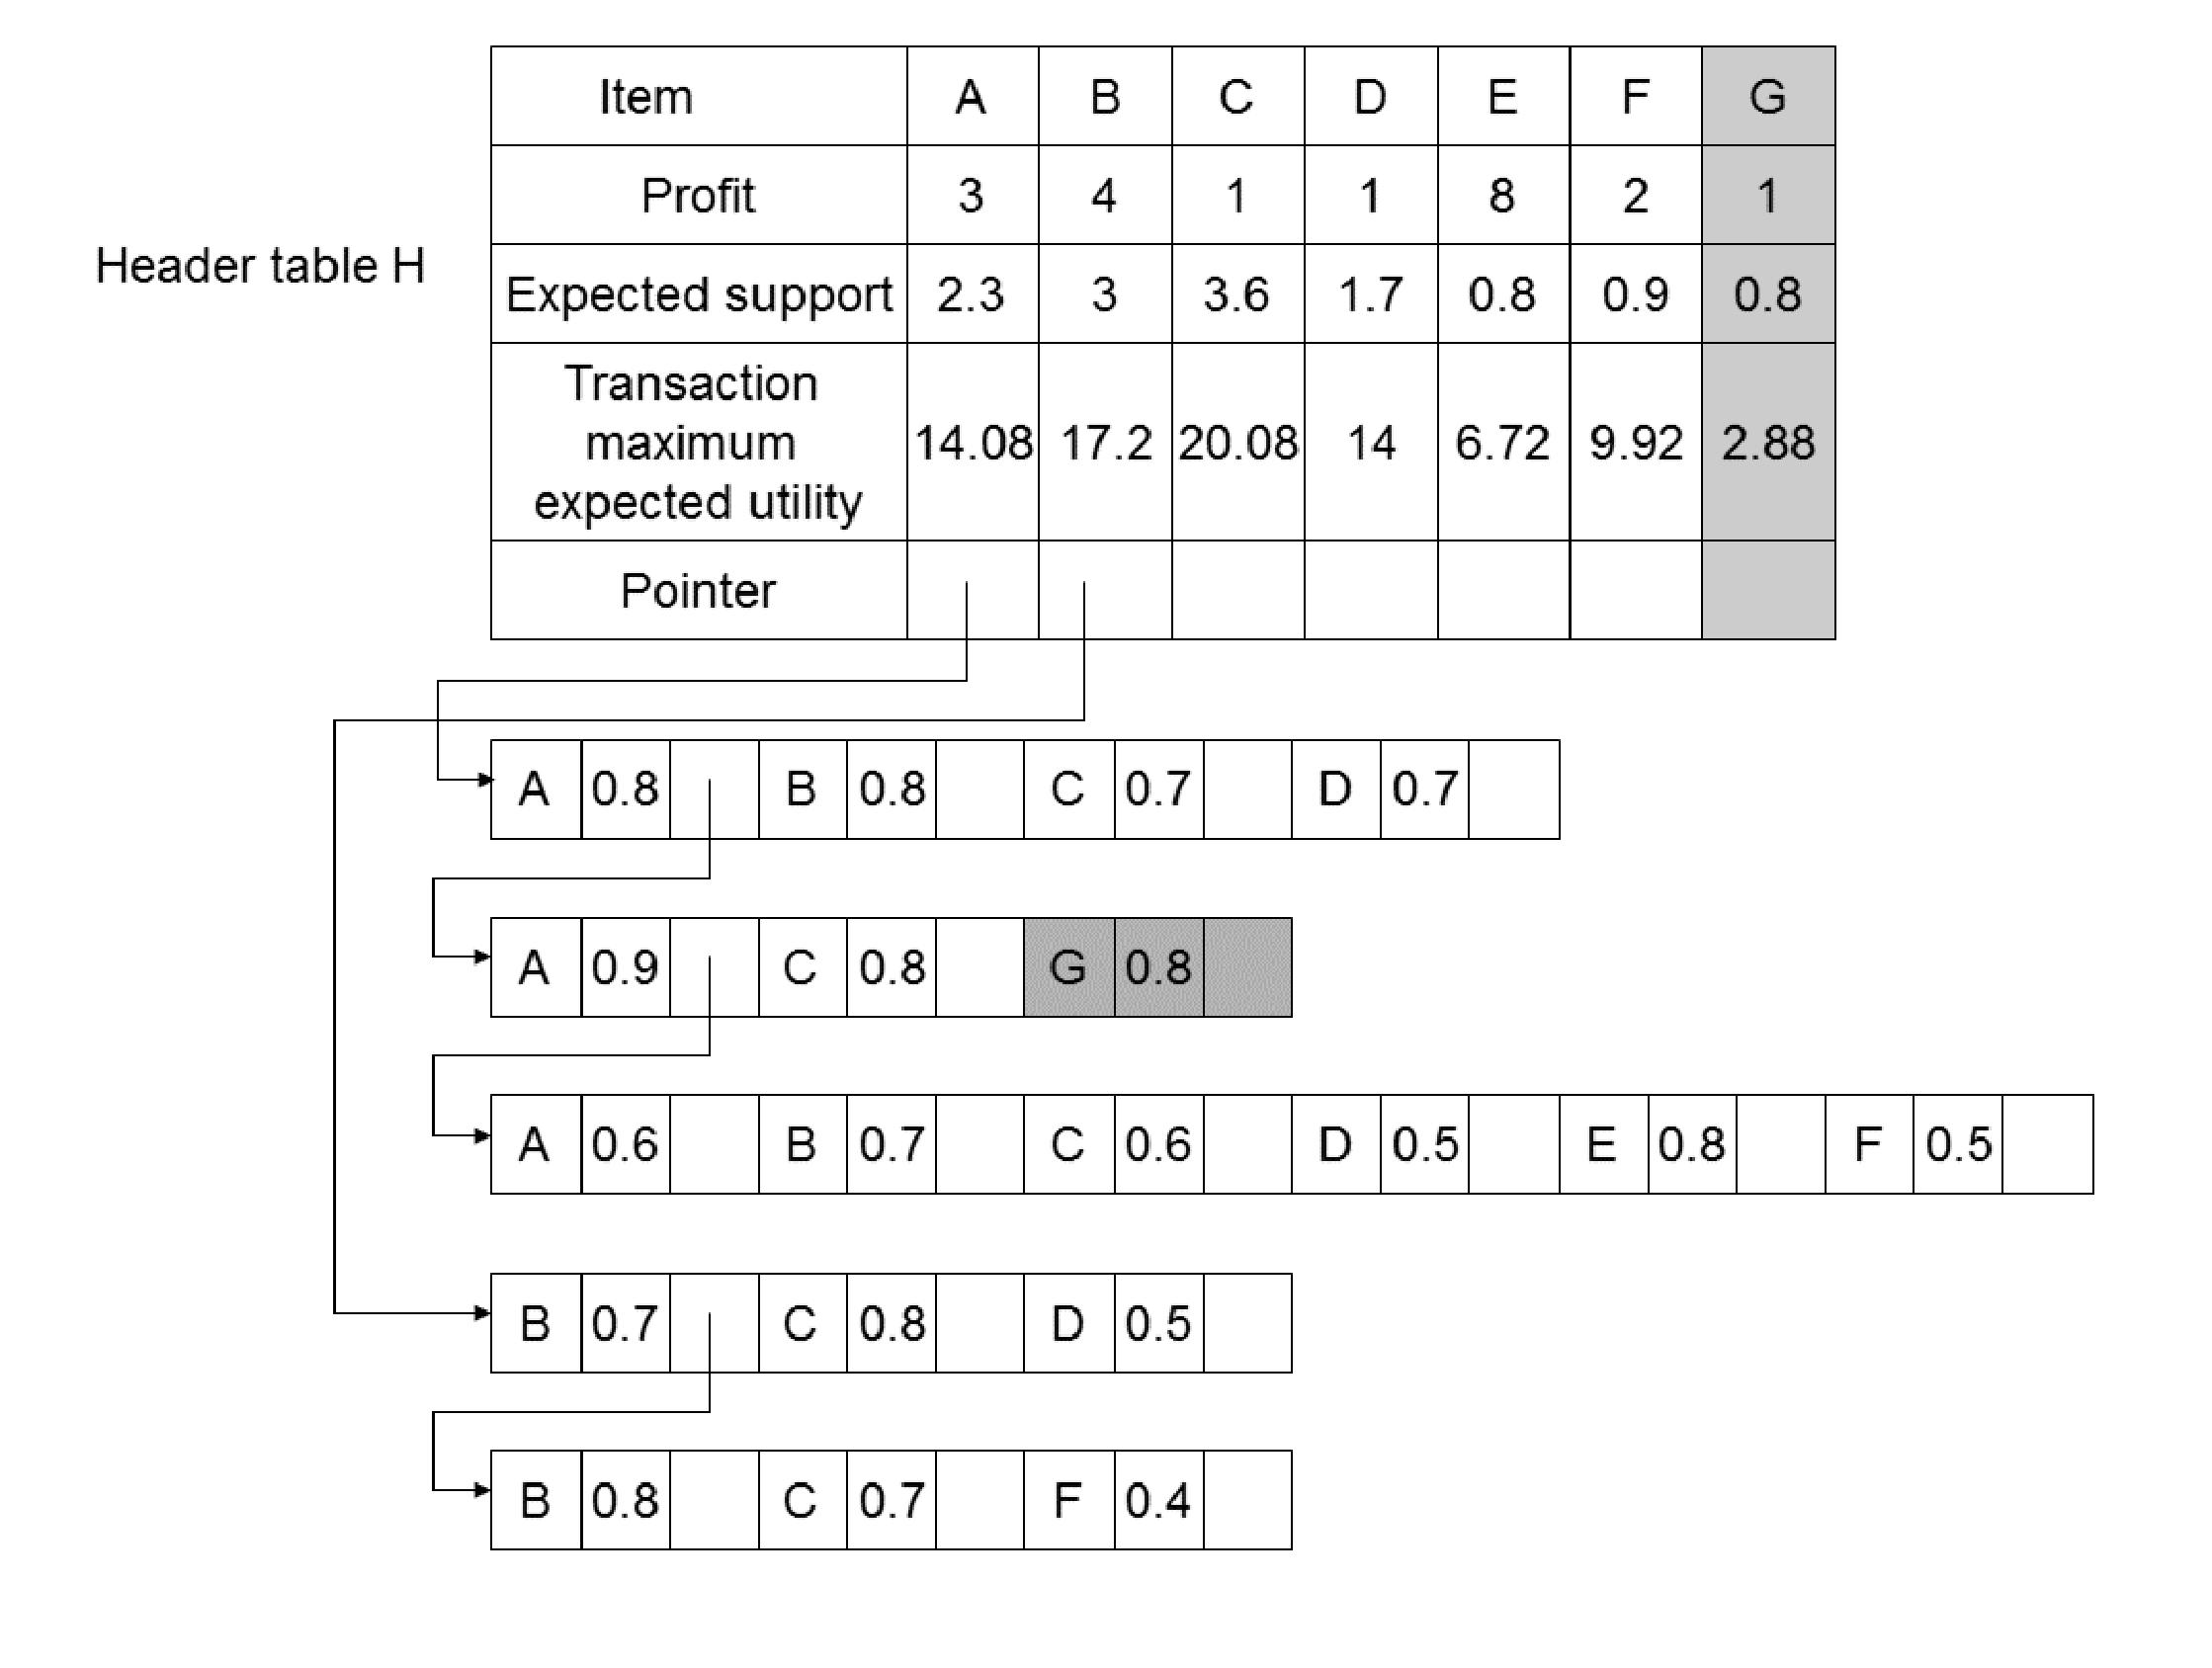
\includegraphics[width=0.99\textwidth]{4.eps}\\
  \caption{UUH-mine data structure with optimization}
  \label{fig4}
\end{figure}

We can derive Theorem 2 through definitions above:


\vspace{-0.3cm}
\begin{theorem}
\label{MUB}
The transaction maximum expected utilities of X's super-itemsets are not more than the transaction maximum expected utilities of X. For $X \subseteq X'$, always $MU(X') \geq MU(X)$.
\end{theorem}
\vspace{-0.3cm}

\begin{proof}
\label{pro:mux}
According to the Chernoff bound, suppose $X_1,X_2,...,X_n$ be independent random variables taking values in \{0,1\}. Let X denote their sum and let $\mu = E[X]$ denote the sum's expected value. For any $\delta > 0$ it holds that
\end{proof}

\begin{equation}
\label{eq:pux}
Pr(X > (1 + \delta)\mu)<(\frac{e^\delta}{(1+\delta)^(1+\delta)})^\mu (\delta > 0)
\end{equation}

In the problem of mining probabilistic high utility itemsets, for one itemset X, its appearance in one uncertain transaction T can be seen as an independent Possion experiment, and the real support of X, i.e. the sup(X) is the sum of many Possion experiments, so the expect of that variable is expected suppprt count of X. The utility probability of X is:

\begin{equation}
\label{eq:prx}
Pr(sup(X)\times U(X)\geq min\_util) = Pr(sup(X)\geq \frac{min\_util}{U(I)})
\end{equation}

When $esup(X) < \frac{min\_util}{U(X)}$, we can let $(1+ \delta) esup(X) = \frac{min\_util}{U(X)}$, so we can get $\delta = \frac{min\_util}{U(X)esup(X)}-1 = \frac{min\_util}{EU(X)} - 1$

\begin{equation}
\label{eq:pru}
Pr(sup(X) \geq \frac{min\_util}{U(X)} )<(\frac{e^\delta}{(1+\delta)^{(1+\delta)}})^{esup(X)}
\end{equation}

While $\delta = \frac{min\_util}{EU(X)} - 1$. The right side of inequality is a decreasing function of $\delta$, so when $\delta$ decreases, the original inequality still holds. Hence we can get the following Lemma:

\vspace{-0.3cm}
\begin{lemma}
\label{lem:lo}
For itemset X, given uncertain transaction database $UD$, utility threshold $min\_util$ and probabilistic high utility threshold $put$ , if $MU(X) < min\_util$ and $(\frac{e^\delta}{(1+\delta)^(1+\delta)})^{esup(X)} < put$, then itemset X and all of its super-itemsets cannot be utility.
\end{lemma}
\vspace{-0.3cm}

Lemma 1 is key point to solve the ��mining probabilistic high utility itemsets�� problem in uncertain database, it can greatly reduce the search space so that the algorithm can be efficient.

We can use it to optimize the UUH-mine framework mentioned in last section, as shown in Fig.4. Because the transaction maximum expected utility of itemset G is 2.88 and cannot pass the check in Lemma 1, G and all of its�� super itemsets cannot be high utility itemsets and we do not need to check them.

We can use the same method to optimize the other header tables generated by projection databases (such as $H_A$, $H_{AB}$, etc).

\vspace{-0.2cm}
\subsection{UUIM Algorithm}
\label{sec:sec:DijSampling}
\vspace{-0.1cm}

In this section, we will introduce UUIM (Uncertain Utility Itemsets Mining) algorithm in detail. First, we will give the overall outline of this algorithm, which divides the mining process into two phases, and then briefly describe them. Then we will explain the two phases in detail.

\begin{algorithm}[htbp]
  \small{
  \caption{\small{UUIM Algorithm}}
  \label{alg:uuim}
  \KwIn{uncertain transaction database $ UD $, utility threshold $ minutil $, probabilistic utility threshold $ put $}
  \KwOut{set of utility itemset $ UIS $}
  $UIS \xleftarrow{} \varnothing$ \;
  \emph{H $\xleftarrow{}$ InitializeHeader(UD, minutil, put)}\;
    \emph{Recursion(H, UD, minutil, put, UIS)}\;
  return UIS}
\end{algorithm}

Algorithm 1(UUIM) is the algorithm framework of mining utility itemsets. This algorithm aims to mine all utility itemsets UIS from the given uncertain transaction database $UD$ through the given utility threshold $min\_util$ and probabilistic high utility threshold $put$. Line 1 is used to initialize the result set UIS; line 2 creates the initial header table H of the UUH-mine framework through function Initialize Header; line 3 uses the key function Recursion to search each items in depth first way; the last line return the calculation results which are all utility itemsets. According to this we can know that the main part of this algorithm consists of two parts, one for creating header table which is explained above in detail; the other is the recursive function Recursion which is used to traverse all probabilistic high utility itemsets.

Next, we will introduce how the key function Recursion works. In algorithm 2(Recursion), line 1 traverses each itemset in the header table; lines 2-3 check whether the new itemset is utility itemset. If it is true it will be added to result; line 4 checks whether that the new itemset can pass the $Pr(sup(X) \geq \frac{min\_util}{U(X)} )<(\frac{e^\delta}{(1+\delta)^(1+\delta)})^{esup(X)}$. If so, a header table will be created in line 5 and traversed in line 6.

\vspace{-0.5cm}
\begin{algorithm}[htbp]
  \small{
  \caption{\small{Recursion Algorithm}}
  \label{alg:recursion}
  \KwIn{header table $ H_{I} $, uncertain transaction database $ UD $, utility threshold $ minutil $, probabilistic utility threshold $ put $, current set of utility itemset $ UIS $}
  \KwOut{updated set of utility itemset $ UIS $}
  \For{each $ i $ in $ H_{I} $ do}{
  \If{$ I\cup{i} $ is utility itemset do}{
    $ UIS=UIS\cup{I\cup{i}} $
  }
  \If{ChernoffCheck($  $) = true do}{
    \emph{create new header table $ H_{I\cup{i}} $}\;
    \emph{Recursion($ H, UD, minutil, put, UIS $)}\;
  }
  }
  End;}
\end{algorithm}
\vspace{-0.9cm}


\section{Performance Evaluations}
\label{sec:exp}
\vspace{-0.2cm}

In this section, we present a performance comparison of UUIM algorithm with the UUIM-Noch algorithm without using the Chernoff pruning strategy. We test the effective of the two algorithms by running time and the memory cost. Finally, we report and analyze our experiment results. All the experiments are conducted on a PC with CPU Inter(R) Core(TM)i5-M450, frequency 2.40GHz, memory 4.00GB, hard disk 500GB. The Operation System is Microsoft Windows 7 Enterprise Edition. The development software is Microsoft Visual Studio 2010, using C++ and its standard template library.

\vspace{-0.5cm}
\subsection{The Datasets}
\label{sec:exp:dataset}
\vspace{-0.1cm}

Three real datasets are used in this paper. We use the classical transaction database Mushroom, and assign probability to transactions in real certain transaction database to get an uncertain database. Similarly, we assign value of each item to the uncertain datasets, Connect and Accident. These three datasets have different scales. The numbers of transactions and items are listed in Table~\ref{tab:Rdataset}.


\begin{table}[htbp]
\vspace{-0.2cm}
  \centering
  \caption{\small{Real Dataset Parameters}}
\vspace{-0.1cm}
  \label{tab:Rdataset}
  \begin{tabular}{|c|c|c|}
    \hline
    \bfseries {Name of Dataset} & \bfseries {Transaction Number} & \bfseries {Item Number} \\
    \hline
    Mushroom & 8,124 & 120 \\
    \hline
    Connect & 67,557 & 129 \\
    \hline
    Accident & 340,183 & 468 \\
    \hline
    %soc-Epinions1 & 75,879 & 508,837 \\
%    \hline
    \end{tabular}
\vspace{-0.4cm}
\end{table}

\vspace{-0.3cm}
\subsection{Efficiency evaluation}
\label{sec:exp:alg:time}
\vspace{-0.3cm}

This subsection mainly evaluate the algorithm efficiency. We will evaluate from three angles: change of utility threshold, change of probabilistic utility threshold and whether use Chernoff bound pruning strategy. In order to hold the principle of single variable, the default parameter setting is: default utility threshold $min\_util = 1$, default probabilistic utility threshold put = 0.6. When one of them is changing, the other keep the default value. Moreover, the range of the utility threshold minutil is 0.5 to 1.5 while the range of the probabilistic utility threshold put is 0.5 to 0.9. According these big ranges, we can clearly see the characteristics of UUIM algorithm and UUIM-NoCh algorithm thus the presented experiment results can be more objective.

\begin{figure*}[htbp]
\vspace{-0.7cm}
  \centering
  \subfigure[\small{Mushroom}]{
      \label{fig:time:ol}
      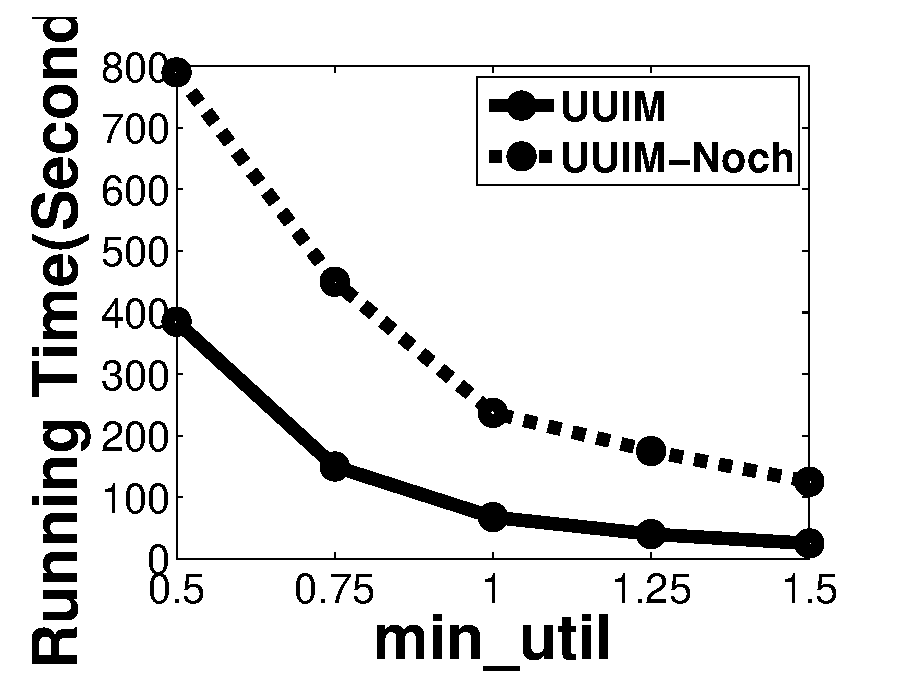
\includegraphics[width=0.32\textwidth]{01.eps}}
  \subfigure[\small{Connect}]{
      \label{fig:time:sf}
      \includegraphics[width=0.32\textwidth]{02.eps}}
  \subfigure[\small{Accident}]{
      \label{fig:time:wiki}
      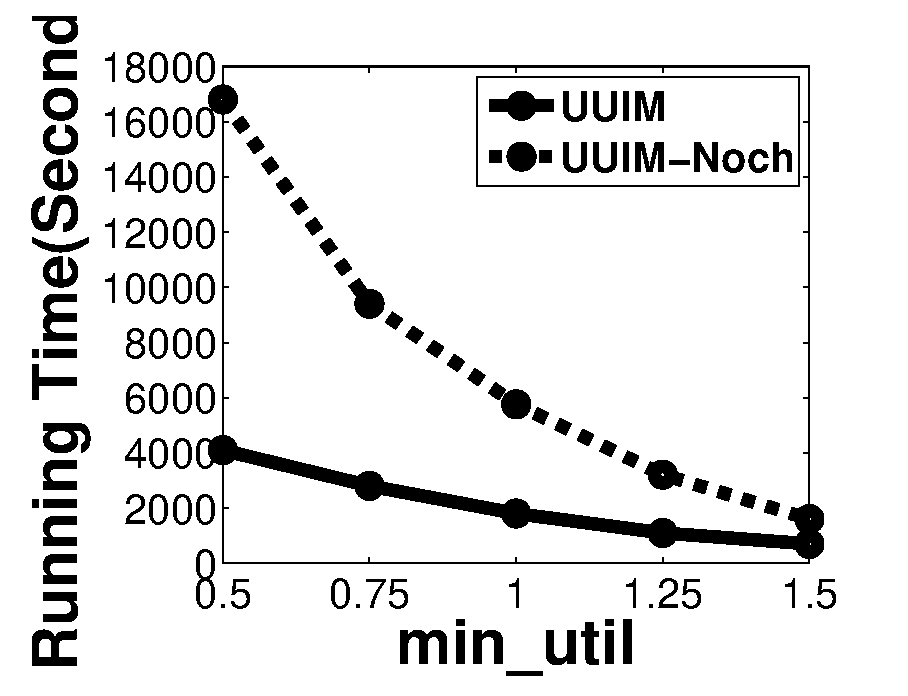
\includegraphics[width=0.32\textwidth]{03.eps}}
  %\subfigure[\small{soc-Epinions1}]{
%      \label{fig:time:soc}
%      \includegraphics[width=0.35\textwidth]{fig-time-Soc.eps}}
\vspace{-0.3cm}
  \caption{Running time vs Minimum Utility Threshold}
  \label{fig:time}
\vspace{-0.6cm}
\end{figure*}

Fig.5 shows the comparison of UUIM algorithm and UUIM-NoCh algorithm with different utility thresholds in three different datasets. Clearly, in the same parameter setting the efficiency of UUIM algorithm is about two times more than the efficiency of UUIM-NoCh algorithm. The difference becomes larger as the utility threshold goes lower. At the same time, the larger is the scale of datasets, the UUIM algorithm shows the better. This shows that the Chernoff bound pruning strategy can efficiently reduce the search space, greatly decrease the number of itemsets need to be calculated, thus greatly increase the algorithm efficiency.

\begin{figure*}[htbp]
\vspace{-0.5cm}
  \centering
  \subfigure[\small{Mushroom}]{
      \label{fig:memory:ol}
      \includegraphics[width=0.32\textwidth]{04.eps}}
  \subfigure[\small{Connect}]{
      \label{fig:memory:sf}
      \includegraphics[width=0.32\textwidth]{05.eps}}
  \subfigure[\small{Accident}]{
      \label{fig:memory:wiki}
      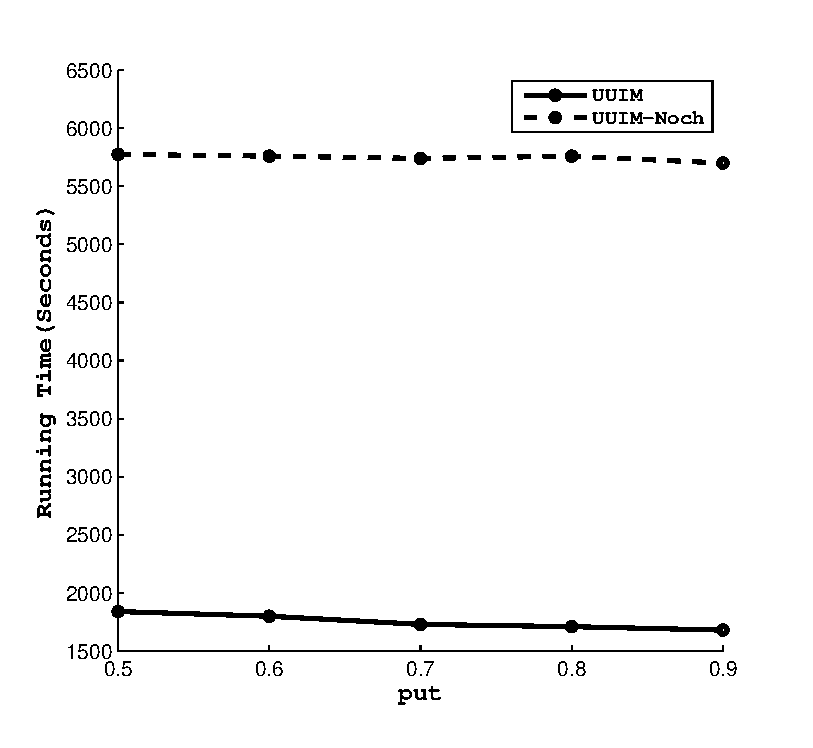
\includegraphics[width=0.32\textwidth]{06.eps}}
  %\subfigure[\small{soc-Epinions1}]{
%      \label{fig:memory:soc}
%      \includegraphics[width=0.4\textwidth]{fig-mem-Soc.eps}}
\vspace{-0.3cm}
  \caption{Running time vs Probabilistic Utility Threshold}
  \label{fig:memory}
\vspace{-0.6cm}
\end{figure*}

Then we test the influence of the change of probabilistic utility threshold to UUIM algorithm and UUIM-NoCh algorithm. Fig.6 shows that while the probabilistic utility goes higher, the running time of UUIM-NoCh left largely unchanged, but the running time of UUIM algorithm is decreasing. Thus shows that while the probabilistic utility threshold gets higher, the effect of Chernoff bound pruning strategy will be little better, but it does not merely influence UUIM-NoCh algorithm.

\vspace{-0.3cm}
\subsection{Memory Cost}
\label{sec:exp:memory}
\vspace{-0.2cm}

Similar to the aforementioned experiments, the default utility threshold is $min\_util=1.0$ and the default probabilistic utility threshold is put=0.6. The range of the utility threshold is 0.5 to 1.5 while the range of the probabilistic utility threshold is 0.5 to 0.9.

\begin{figure*}[htbp]
\vspace{-0.7cm}
  \centering
  \subfigure[\small{Mushroom}]{
      \label{fig:mse:ol}
      \includegraphics[width=0.28\textwidth]{07.eps}}
  \subfigure[\small{Connect}]{
      \label{fig:mse:sf}
      \includegraphics[width=0.32\textwidth]{08.eps}}
  \subfigure[\small{Accident}]{
      \label{fig:mse:wiki}
      \includegraphics[width=0.32\textwidth]{09.eps}}
  %\subfigure[\small{soc-Epinions1}]{
%      \label{fig:mse:soc}
%      \includegraphics[width=0.4\textwidth]{fig-var-Soc.eps}}
\vspace{-0.3cm}
  \caption{Memory Cost vs Minimum Utility Threshold}
  \label{fig:mse}
\vspace{-0.6cm}
\end{figure*}

Fig.7 shows the comparison of UUIM and UUIM-NoCh on three datasets. We can see that while the utility threshold goes higher, the memory cost of these two algorithms decreases, and the difference between UUIM and UUIM-NoCh is very small, hence we can conclude that the operation of adding transaction maximum utility to header table doesn't have obvious effect.

\begin{figure*}[htbp]
\vspace{-0.3cm}
  \centering
  \subfigure[\small{Mushroom}]{
      \label{fig:error:ol}
      \includegraphics[width=0.32\textwidth]{10.eps}}
  \subfigure[\small{Connect}]{
      \label{fig:error:sf}
      \includegraphics[width=0.25\textwidth]{11.eps}}
  \subfigure[\small{Accident}]{
      \label{fig:error:wiki}
      \includegraphics[width=0.32\textwidth]{12.eps}}
  %\subfigure[\small{soc-Epinions1}]{
%      \label{fig:error:soc}
%      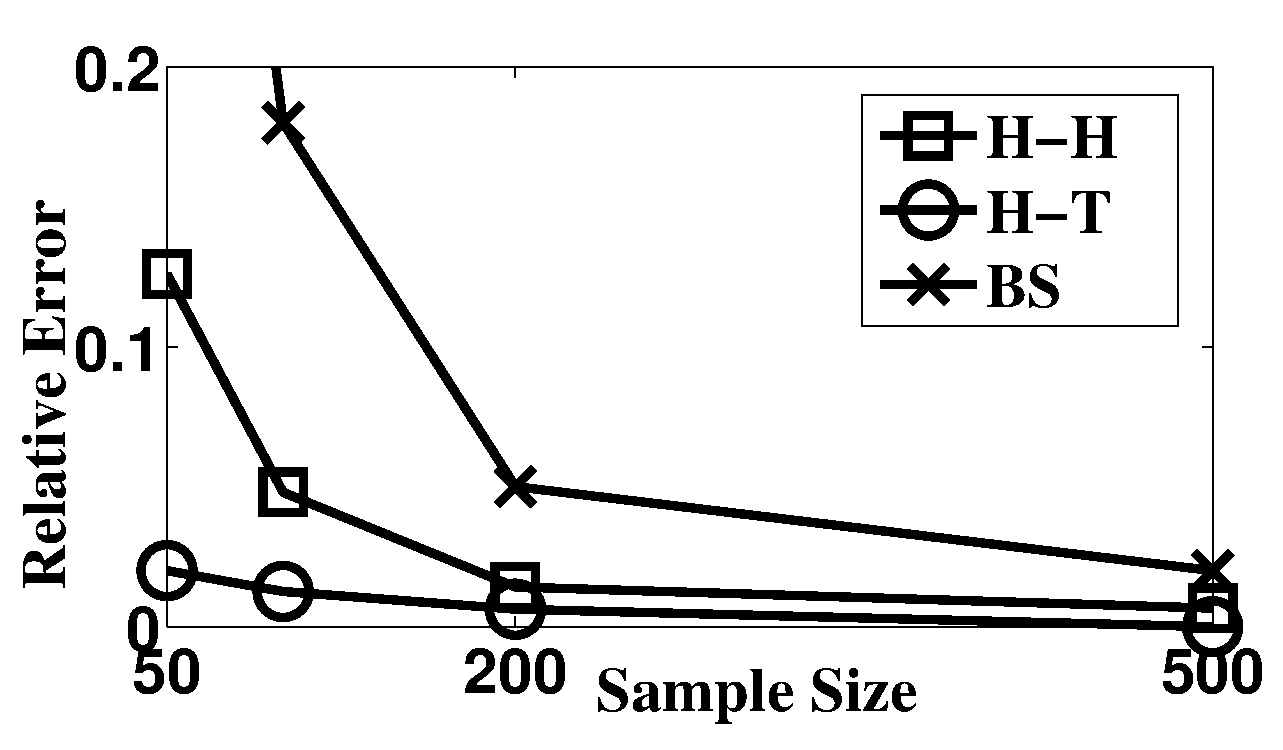
\includegraphics[width=0.4\textwidth]{fig-err-Soc.eps}}
\vspace{-0.3cm}
  \caption{Memory Cost vs Probabilistic Utility Threshold}
  \label{fig:error}
\vspace{-0.3cm}
\end{figure*}

Fig.8 shows the memory cost of UUIM and UUIM-NoCh in different probabilistic utility threshold. It shows that probabilistic utility threshold has almost no effect on memory cost. Besides, there is no difference between the memory cost of two algorithms.

\subsection{Experimental Summary}

In the efficiency evaluation, we can clearly see that the efficiency of UUIM algorithm is much more than UUIM-NoCh, and the difference get bigger while the utility threshold and the probabilistic utility threshold goes higher. In the cost evaluation, we can see that two algorithms need same memory in different utility threshold and probabilistic utility threshold. Thus the Chernoff bound pruning strategy does not decrease the memory cost. In summary, the proposed UUIM algorithm is obviously better than the baseline algorithm.

\vspace{-0.4cm}
\section{Related Work}
\label{sec:related}
In this section, we review the related work in two categories, mining high utility itemsets in deterministic data and mining frequent itemsets in uncertain data.

\vspace{-0.2cm}
\subsection{Deterministic High Utility Itemset Mining}
Since Rakesh Agrawal first proposed the concept of mining frequent itemsets (or called mining large itemset) \cite{DBLP:conf/vldb/AgrawalS94}, many efficient algorithms about mining frequent itemsets have been designed, such as FP-growth \cite{DBLP:conf/sigmod/HanPY00}, Eclat \cite{DBLP:journals/tkde/Zaki00}, and so on.

Especially, utility itemset mining, also generally called utility pattern mining, was first introduced in \cite{DBLP:conf/icdm/ChanYS03,DBLP:conf/sdm/YaoHB04}. Although the UMining algorithm was proposed by \cite{DBLP:conf/sdm/YaoHB04}, it cannot extract the complete set of them. A transaction-weighted downward closure property was introduced in \cite{DBLP:conf/pakdd/LiuLC05}, in which a two-phase algorithm was proposed and performed faster than UMining. Moreover, IHUP \cite{DBLP:journals/tkde/AhmedTJL09} maintains the high utility patterns in an incremental environment; since it avoids multiple scans of the database, its efficiency is far better than \cite{DBLP:conf/pakdd/LiuLC05}. Recently, UP-Growth \cite{DBLP:conf/kdd/TsengWSY10,DBLP:journals/tkde/TsengSWY13} also proposed a tree structure, UP-Tree, to mine high utility itemsets. Compared to IHUP, UP-Growth is more efficient, since it further reduces the number of promising patterns which cannot be pruned in IHUP. Furthermore, several variants, such as mining top-$k$ utility itemsets \cite{DBLP:conf/kdd/WuSTY12}, mining the concise and lossless representative high utility patterns \cite{DBLP:conf/icdm/WuFYT11,DBLP:journals/tkde/TsengWFY15}, and mining big high utility itemsets \cite{DBLP:conf/pakdd/LinWT15}, were proposed recently.

%To solve such problem, some alternative approaches were proposed instead of mining complete frequent itemsets, such as mining frequent closed itemsets \cite{DBLP:conf/icdt/PasquierBTL99}, mining frequent maximal itemsets \cite{DBLP:conf/sigmod/Bayardo98}, mining non-derivable frequent itemsets \cite{DBLP:conf/pkdd/CaldersG02}, etc. These alternative methods can be grouped into two categories: the lossless compression-based methods and lossy compression-based methods. Among above approaches, mining frequent closed and non-derivable itemsets are lossless compression-based methods. The others belong to the lossy compression-based methods. Moreover, even though there are a lot of studies on mining frequent itemsets, all these approaches do not concern the correlated property of uncertain data.
\vspace{-0.2cm}
\subsection{Uncertain Frequent Itemset Mining}
Another set of related researches with our work is the issues of mining frequent itemsets over uncertain data. Different from the certain case, the definition of a frequent itemset in uncertain data has two types of probabilistic semantics: \textit{expected support-based frequent itemset} \cite{DBLP:conf/kdd/AggarwalLWW09,DBLP:conf/pakdd/ChuiKH07} and \textit{probabilistic frequent itemset} \cite{DBLP:conf/kdd/BerneckerKRVZ09}. In the definition of the expected support-based frequent itemset, the expectation of the support of an itemset is defined as the measurement, called as the expected support of this itemset \cite{DBLP:conf/kdd/AggarwalLWW09,DBLP:conf/pakdd/ChuiK08,DBLP:conf/pakdd/ChuiKH07,DBLP:conf/pakdd/LeungMB08}. In the definition of probabilistic frequent itemset \cite{DBLP:conf/kdd/BerneckerKRVZ09,DBLP:conf/kdd/SunCCC10,DBLP:conf/cikm/WangCLC10}, the probability that an itemset appears at least the minimum support (\textit{min\_sup}) times is defined as the measurement, called as the frequent probability of an itemset. Recently, \cite{DBLP:journals/pvldb/TongCCY12} using an experimental method shows the aforementioned two definitions of uncertain frequent itemsets is actually equivalent while the uncertain databases are very large.

Although there are related researches of mining frequent itemsets over uncertain data, all of them are built over the assumption that each item has no unit profit and only appear once in each transaction. In other words, none of existing work cannot address the problem of mining probabilistic high utility itemsets over uncertain data.

\section{Conclusion}

In this paper, we formulate a new type of problem of mining uncertain frequent itemsets, called \textit{\underline{m}ining \underline{p}robabilistic \underline{h}igh \underline{u}tility itemsets in uncertain databases} (MPHU), where each item has an unit profit and likely appears multiple times in one transaction. In order to solve the \textit{MPHU} problem, we propose a novel mining framework, called \textit{UUIM}, which not only includes an efficient mining algorithm but also contains an effective pruning technique. Extensive experiments on both real and synthetic datasets verify the effectiveness and efficiency of proposed solutions.

\bibliographystyle{splncs03}
\bibliography{cup}

\end{document}
